\subsection{Full Yukawa Results}
\label{sec:yukawa_results}

Here, we examine the spacetime cost to block-encode the full Yukawa model which includes interactions between fermionic, antifermionic, and bosonic modes.  
This is a theory of interacting fermions and bosons which can be used as a model of the strong nuclear force between hadrons.
The Lagrangian for this model is given as:
\begin{equation}
    \label{eq:yukawa-lagrangian}
    \mathcal{L} = \bar \psi \left(i\gamma^\mu \partial_\mu - m \right)\psi + \frac{1}{2}\partial_\mu \phi \partial^\mu \phi - \frac{1}{2}\mu^2\phi^2 - g\bar \psi \psi \phi,
\end{equation}
where $m_f$ is the mass of the fermion, $m_b$ is the mass of the boson, and $g$ describes the strength of the interaction.
Unlike $\phi^4$ theory, the Yukawa model involves multiple types of fields including a fermionic (Dirac) field ($\psi$) and the conjugate (antifermionic) Dirac ($\bar \psi$) field, in addition to the bosonic field ($\phi$).

The Hamiltonian associated with this Lagrangian can be written in second-quantization as:
\begin{align}
    \begin{split}
        H = &\sum_i c_i b_i^\dagger b_i + \sum_i c_i d_i^\dagger d_i + \sum_i c_i a_i^\dagger a_i + \\
        &\sum_{ijk}c_{ijk}\left(b_i^\dagger b_j a_k^\dagger + h.c. \right) + \sum_{ijk}c_{ijk}\left(d_i^\dagger d_j a_k^\dagger + h.c. \right) + \\
        &\sum_{ijk}c_{ijk}\left(b_i^\dagger d_j^\dagger a_k + h.c. \right) + \sum_{ijkl}c_{ijkl}b_i^\dagger b_j a_k^\dagger a_l + \\
        &\sum_{ijkl}c_{ijkl}d_i^\dagger d_j a_k^\dagger a_l + \sum_{ijkl}c_{ijkl}\left(b_i^\dagger d_j^\dagger a_k a_l + h.c. \right)
    \end{split}
\end{align}
where the values of the coefficients can be determined by classical preprocessing.

\begin{figure*}
    \label{fig:full-yukawa}
    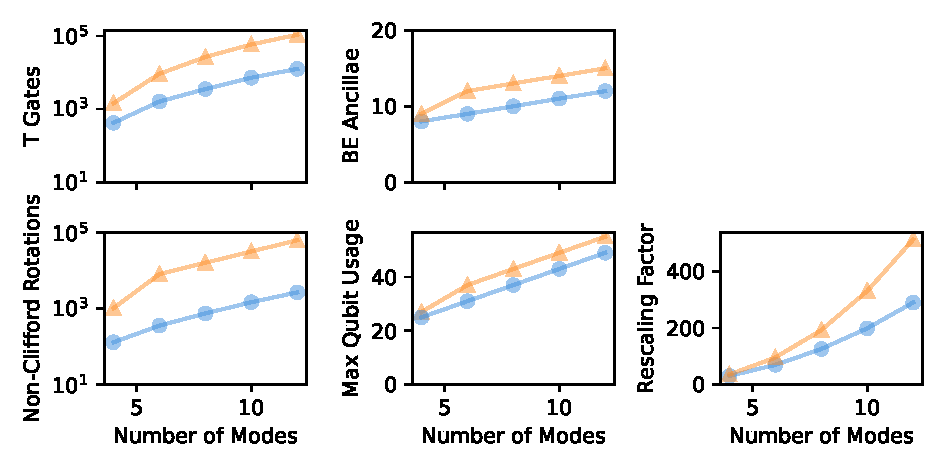
\includegraphics[width = 16cm]{figures/full-yukawa-resolution-3.pdf}
    \caption{
        \textbf{Full Yukawa}
        The number of T gates (upper-left), number of non-Clifford rotations (lower-left), block-encoding ancillae (upper-middle), maximum number of qubits used (lower-middle), and rescaling factor (lower-right) are shown as a function of the number of momentum modes.
        The bosonic cutoff is fixed to $\Omega = 3$ and the parameters $m_f$, $m_b$, and $g$ are set to $1$ for all data points.
        Results for the ``Pauli - Expansion" method are shown as the orange triangles and results for LOBE are shown as the blue circles.
        The optimal rescaling factor, which is given by the L2 norm of the Hamiltonian, is shown as the dashed black crosses.
    }
\end{figure*}

In Figure \ref{fig:full-yukawa}, the spacetime costs for both the Pauli Expansion and LOBE block-encodings are shown as a function of the number of momentum modes.
For this model, the LOBE constructions result in fewer required quantum resources for all metrics.
Notably, the number of T gates and number of non-Clifford rotations required for LOBE is approximately two orders of magnitude smaller than the Pauli Expansion construction when the number of modes is $12$.
